\documentclass[conference]{IEEEtran}
\usepackage{amsmath,amssymb}
\usepackage{booktabs}
\usepackage{url}
\usepackage{graphicx}
\graphicspath{{../results/figures/}}

\begin{document}

\title{Projected Quantum Kernels and the Geometric Test for Advantage\\
\large AI 631 Quantum Machine Learning, Fall 2026 --- Project \#6\\
Report draft, Week 3 (November 29, 2026)}

\author{\IEEEauthorblockN{Farrukh Shahzad (25280034), Shams ul Arifeen (25280080), Haider Nadeem (25280003)}
\IEEEauthorblockA{Lahore University of Management Sciences (LUMS)\\
Code: \url{https://github.com/ifarrukhshahzad/AI631-Projected-Quantum-Kernels}}}

\maketitle

\begin{abstract}
Huang \textit{et al.}~\cite{huang2021} proposed the geometric difference $g$ as a data-dependent indicator of when a quantum kernel can outperform a classical one, and introduced projected quantum kernels built from one-qubit reduced density matrices. We test these ideas at small scale on PCA-reduced Fashion-MNIST (T-shirt/top vs.\ Shirt), comparing fidelity and projected quantum kernels with tuned classical models under matched per-model tuning budgets, over 5 seeds and 2--8 qubits, in simulation, under a noise model of an IBM Heron device, and on the real IBM quantum computer \texttt{ibm\_kingston}. On the original labels no quantum kernel meets our improvement criterion, and the best quantum model chosen by cross-validation is below the best classical model at every qubit count, although $g\approx3$ for both quantum kernels. On relabeled data whose labels follow the direction of largest geometric difference (adapted from~\cite{huang2021}), the projected kernel meets our improvement criterion at 6 qubits. This advantage survives the device noise model over all 5 seeds ($\overline{\Delta A}=+0.045$ to $+0.095$). On real hardware (one seed, all 120 images measured) it shrinks from $+0.000/+0.125/+0.100$ to $-0.050/+0.075/+0.025$ for the three label sets, and readout-error mitigation does not recover it. Noise lowers $g$ by 9--13\% for the fidelity kernel but by at most 1.4\% for the projected kernel. We give circuit diagrams of both kernel architectures and a first set of recommendations for QML engineers.
\end{abstract}

\section{Introduction and Motivation}
A support vector machine (SVM) learns a decision boundary using only a kernel $k(x,x')$, a measure of similarity between two data points. A quantum kernel computes this similarity from quantum states prepared by a data-encoding circuit~\cite{schuld2019,havlicek2019}, in a space that grows exponentially with the number of qubits. A large feature space alone, however, does not guarantee better learning. Huang \textit{et al.}~\cite{huang2021} showed that, when enough training data is available, classical models can often match quantum models, and that the \emph{geometric difference} between a classical kernel matrix $K^{C}$ and a quantum kernel matrix $K^{Q}$ helps assess the potential for a prediction advantage. They also introduced \emph{projected quantum kernels}, which compare data points through one-qubit reduced density matrices (1-RDMs) instead of full quantum states. A test that predicts from the data alone whether a quantum kernel can help would be useful in practice, because quantum hardware time is scarce and noisy; kernel classification with such an indicator is therefore a setting where a quantum advantage can be looked for in a controlled way.

\textbf{Research question.} At small scale, is the geometric difference associated with when a fidelity or projected quantum kernel outperforms classical kernels?

\textbf{Sub-questions.} (1) How do fidelity and projected kernels compare with tuned RBF, polynomial and linear kernels on the original labels? (2) How does the geometric difference change with qubit count, and does it track the accuracy gap? (3) Does the advantage indicated by a large geometric difference appear on a relabeled dataset designed to favour the quantum kernel? (4) How much do finite shots, device noise and real hardware change the projected-kernel features and accuracy? (5) Added after the Week~2 feedback: does the advantage found in (3) survive device noise and a real quantum computer?

\section{Background and Problem Setup}
\subsection{Quantum kernels and the geometric difference}
A kernel SVM needs only the $N\times N$ matrix $K_{ij}=k(x_i,x_j)$ of the training points, which must be symmetric and positive semidefinite (PSD). A quantum kernel defines $k$ through a data-encoding circuit $U(x)$, giving $|\psi(x)\rangle=U(x)|0\rangle^{\otimes n}$~\cite{schuld2019,havlicek2019}. The \textbf{fidelity kernel} is
\begin{equation}
k^{Q}(x,x') = |\langle \psi(x)|\psi(x')\rangle|^{2},
\end{equation}
estimated as the probability of measuring all zeros after $U(x')^\dagger U(x)$, with one circuit per \emph{pair} of data points. For the \textbf{projected kernel}, the 1-RDM of qubit $k$ is fixed by its three Pauli expectation values,
\begin{equation}
\rho_k(x)=\tfrac{1}{2}\big(I+\langle X_k\rangle_x X+\langle Y_k\rangle_x Y+\langle Z_k\rangle_x Z\big),
\end{equation}
and the kernel of~\cite{huang2021} is
\begin{equation}
k^{PQ}(x,x') = \exp\!\Big(-\gamma \sum_{k}\big\|\rho_k(x)-\rho_k(x')\big\|_F^{2}\Big),
\end{equation}
where $\|\rho_k(x)-\rho_k(x')\|_F^2=\tfrac{1}{2}\sum_{P\in\{X,Y,Z\}}\big(\langle P_k\rangle_x-\langle P_k\rangle_{x'}\big)^2$. These features are measured once per \emph{sample} and reused for every pair. With both kernels normalised to trace $N$, the \textbf{geometric difference} of~\cite{huang2021} is
\begin{equation}
g(K^{C}\|K^{Q})=\sqrt{\Big\|\sqrt{K^{Q}}\,(K^{C})^{-1}\sqrt{K^{Q}}\Big\|_{\infty}},
\end{equation}
where $\|\cdot\|_\infty$ is the spectral norm. For a fixed pair of kernels it depends only on the inputs, not on the labels; with the tuned best classical model $C^\ast$ (Section~\ref{sec:budget}) it depends on the labels only through which classical kernel is selected. Huang \textit{et al.} use $g$ to assess whether a prediction advantage is possible, and to construct labels on which it is~\cite{huang2021}.

\subsection{Data and protocol}
We use Fashion-MNIST~\cite{xiao2017} (official Zalando Research files), T-shirt/top (label $-1$) vs.\ Shirt (label $+1$), two visually similar classes. Each of 5 seeds $\{0,100,200,300,400\}$ draws a balanced subsample of 40 training and 20 test images per class (80/40); the indices are saved in the repository, so every notebook uses identical splits. The synopsis target of 150/50 per class is not feasible, because the fidelity kernel needs one circuit per pair of images and the larger size has about $12\times$ more pairs. With 40 test images, one image changes accuracy by 0.025. Images are reduced by PCA to $n\in\{2,4,6,8\}$ features ($n$ = number of qubits) and min--max scaled to $[-1,1]$, both fitted on training images only (and reused across the inner folds during tuning; test images never enter them). Hyperparameters are chosen by 5-fold stratified cross-validation inside the training set; the test set is used once per seed and model. As in the course NB11 harness, the main quantum results use \emph{sampled} kernels on Qiskit Aer (2048 shots per circuit); exact statevector values are an ideal reference.

\subsection{Circuit architectures}\label{sec:circ}
Feature $x_i$ is loaded into qubit $i$ by $R_y(\alpha x_i)$, followed by a chain of CNOTs between neighbouring qubits; this block is repeated $L$ times from $|0\rangle^{\otimes n}$ (Fig.~\ref{fig:circ}a). The main setting is $L=2$. $L=1$ is a baseline: for one layer the CNOT block cancels in the overlap, so the fidelity kernel reduces to $\prod_i\cos^2\!\big(\alpha(x_i-x_i')/2\big)$, which is classically easy. $L=2$ is not claimed to give any computational advantage. Both quantum kernels share this circuit and differ in what is measured. The \textbf{fidelity kernel} (Fig.~\ref{fig:circ}b) runs $U(x)$, then $U(x')^\dagger$, and measures all qubits; $k^{Q}(x,x')$ is the frequency of the all-zero outcome. The \textbf{projected kernel} (Fig.~\ref{fig:proj}) runs $U(x)$, changes the basis of every qubit ($Z$: none; $X$: $H$; $Y$: $S^\dagger$ then $H$) and measures all qubits; one circuit per basis gives that Pauli for all qubits at once, so each image needs 3 circuits. On \texttt{ibm\_kingston} every circuit is transpiled to the native gates $R_z$, $\sqrt{X}$, $X$ and CZ (Fig.~\ref{fig:circ}c). After transpilation both kernels use the same number of CZ gates (the two middle CNOT chains of the overlap circuit cancel), but the overlap circuit is deeper, and its circuit and shot counts grow with the number of image \emph{pairs} (Table~\ref{tab:res}). This cost difference is why only the projected kernel could be run on hardware.

\begin{figure*}[t]
\centering
\begin{tabular}{@{}c@{\hspace{6pt}}c@{}}
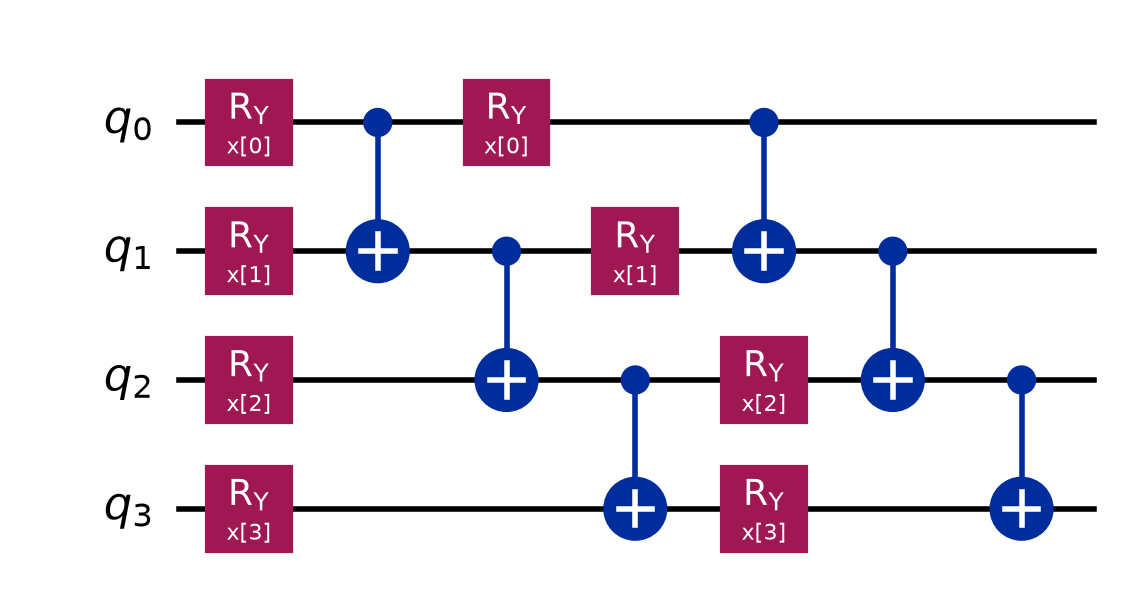
\includegraphics[height=2.6cm]{circuit_encoding.png} &
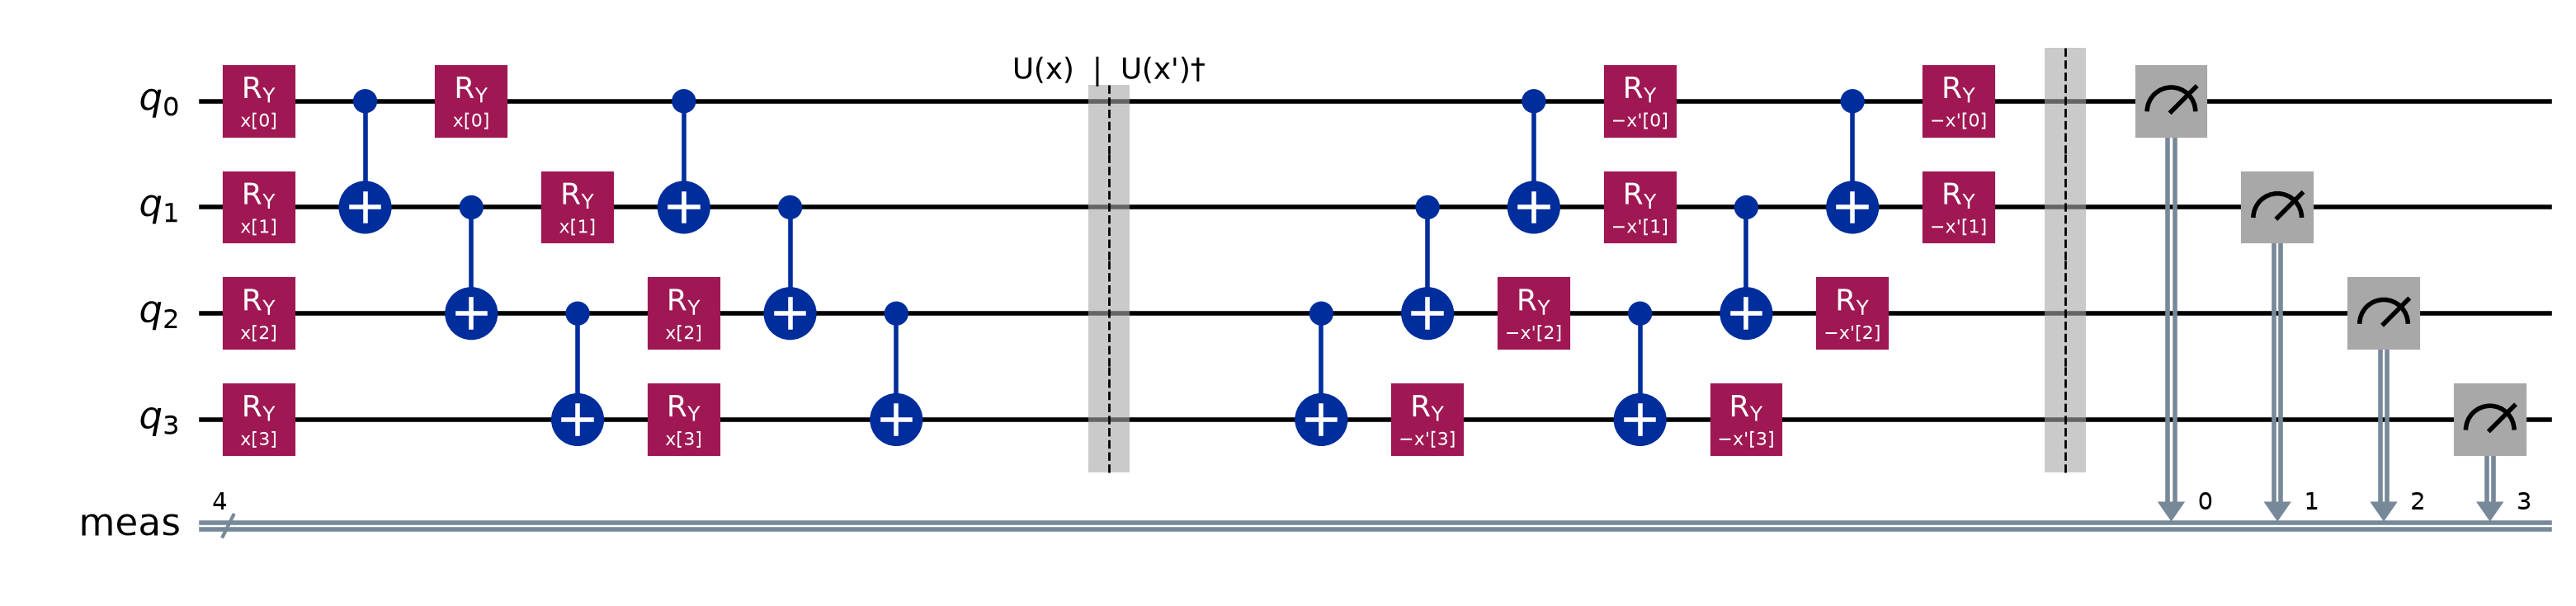
\includegraphics[height=2.6cm]{circuit_fidelity.png}\\
(a) Encoding circuit $U(x)$, $L=2$ & (b) Fidelity kernel: compute--uncompute circuit $U(x')^\dagger U(x)$\\[4pt]
\multicolumn{2}{c}{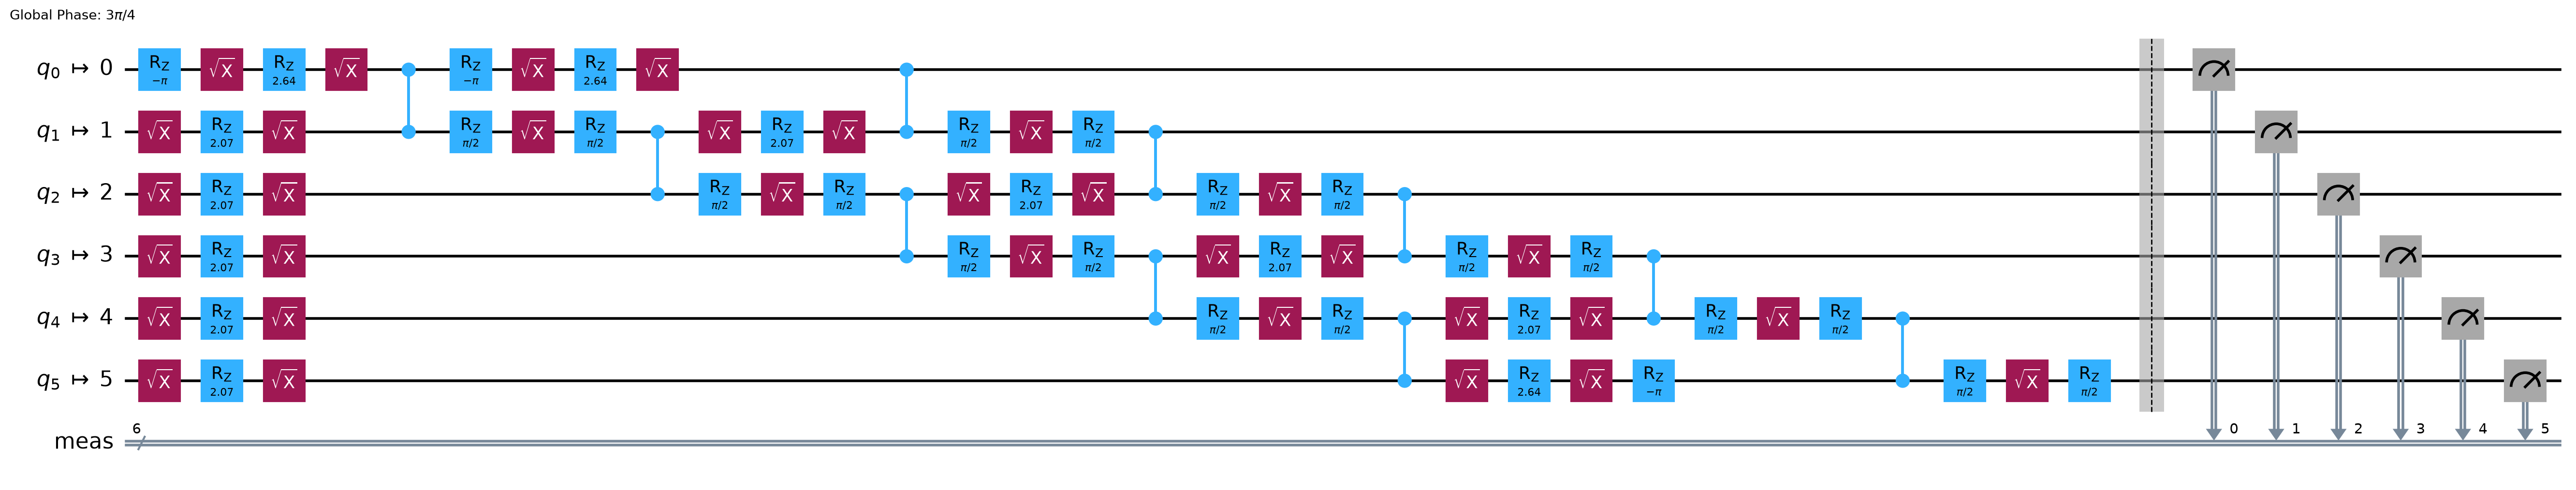
\includegraphics[width=0.86\textwidth]{circuit_projected_transpiled_kingston.png}}\\
\multicolumn{2}{c}{(c) What the hardware runs: projected-kernel $Z$-basis circuit, $n=6$, transpiled to \texttt{ibm\_kingston}: depth 33, 10 CZ}
\end{tabular}
\caption{Circuit architectures, drawn from the code in the repository. (a), (b): $n=4$ for readability (the structure is the same for $n=2,\dots,8$); \texttt{x[i]} and \texttt{x'[i]} are the rotation angles $\alpha x_i$ of the two images, and (b) is checked to be the same unitary as Qiskit's \texttt{unitary\_overlap}, which our code runs. (c): optimisation level 1, generic angles 0.5 so that no gate is removed; each $R_y$ becomes $R_z$ and $\sqrt{X}$ gates and each CNOT a CZ with single-qubit gates around it.}
\label{fig:circ}
\end{figure*}

\begin{figure}[t]
\centering
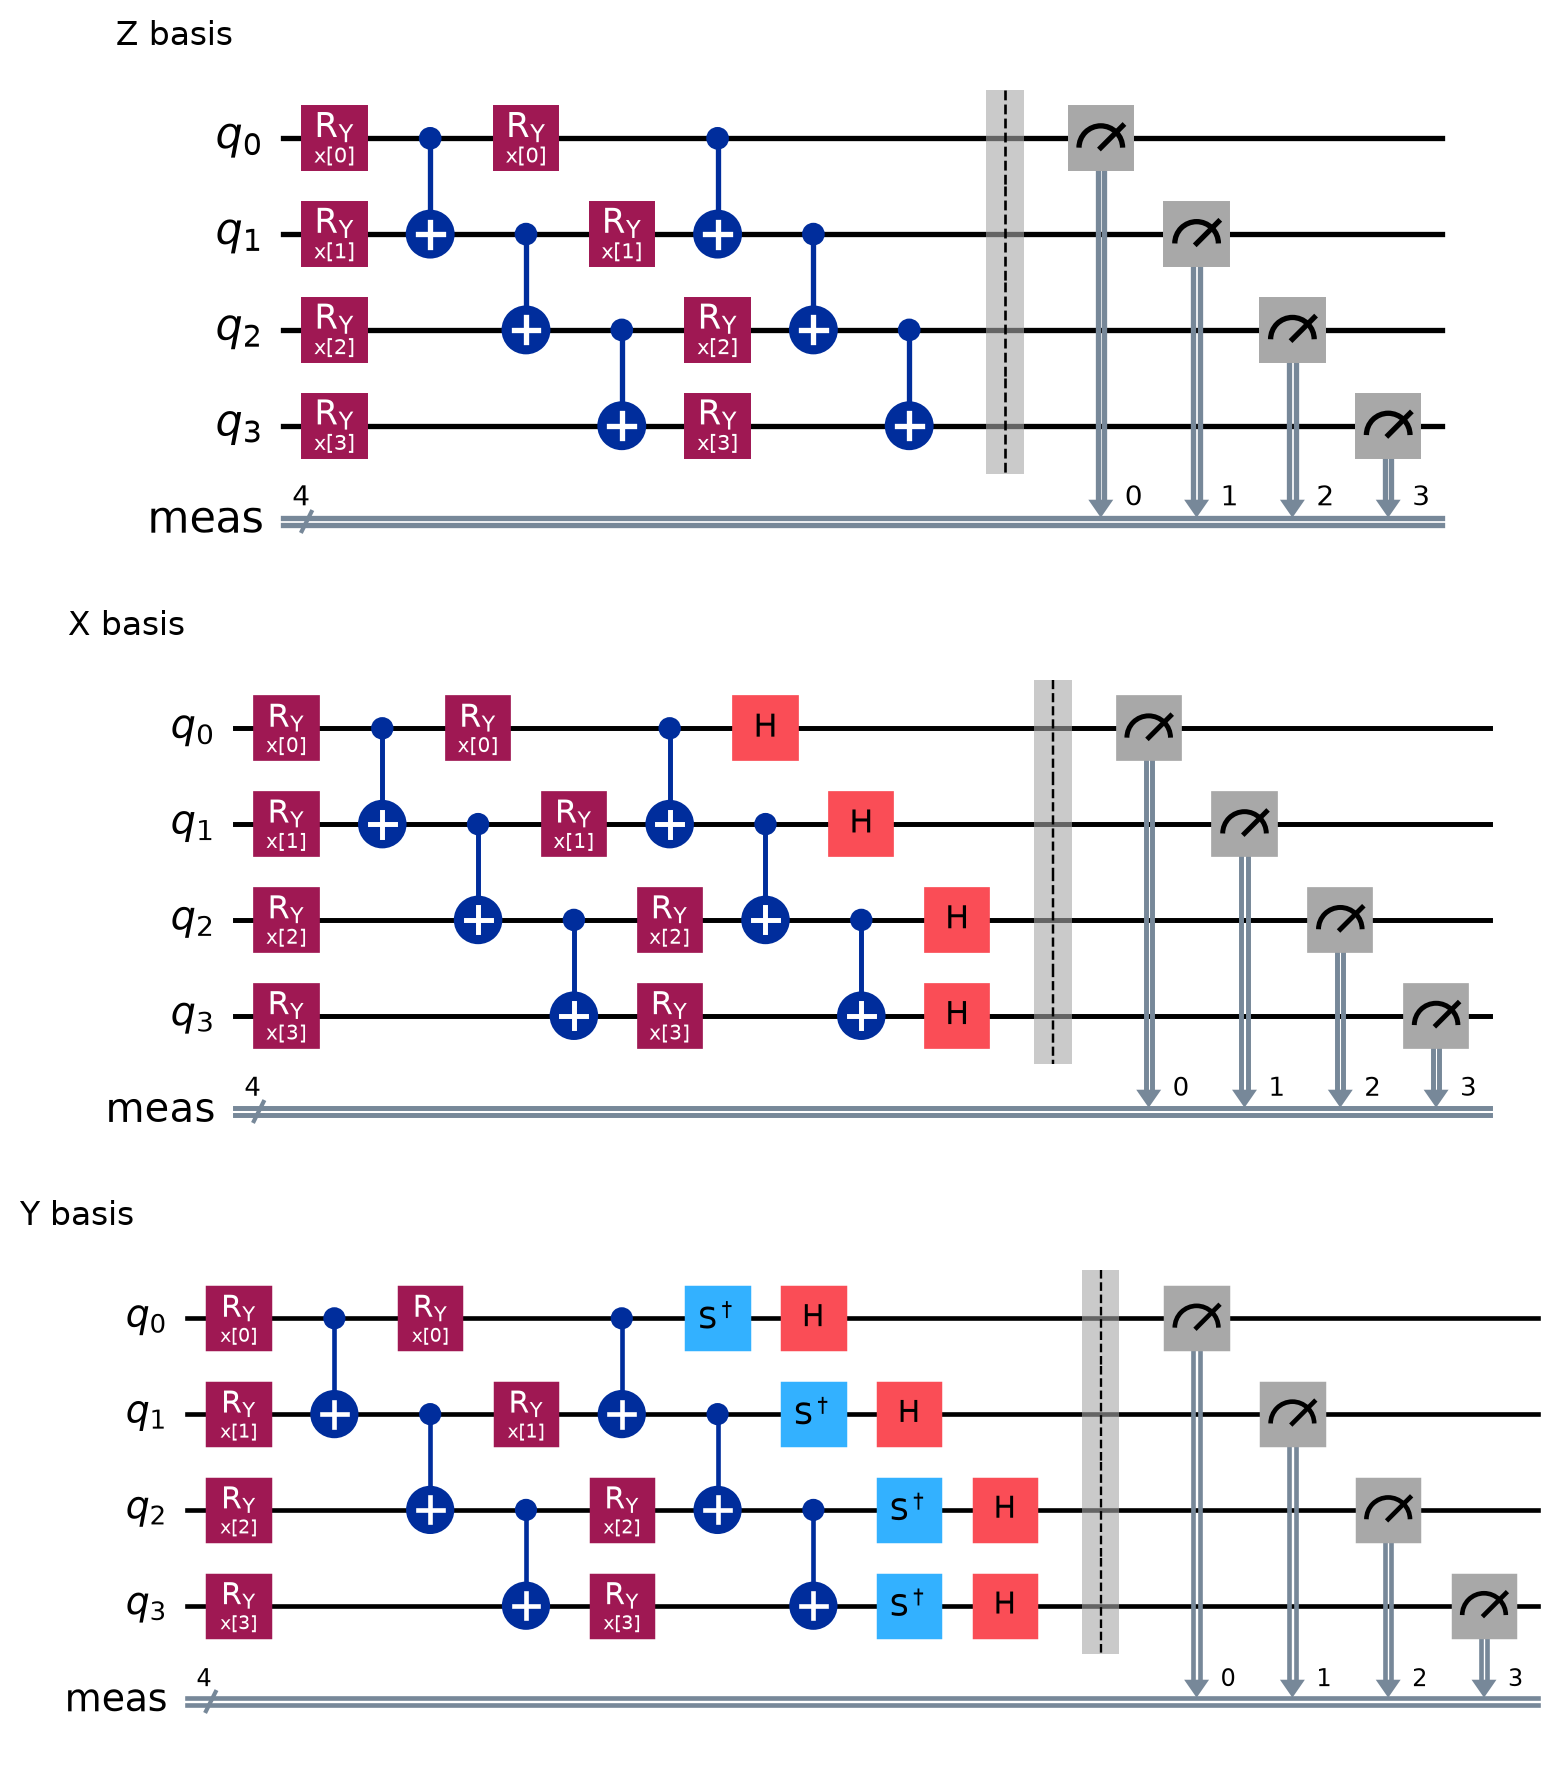
\includegraphics[width=0.8\columnwidth]{circuit_projected.png}
\caption{Projected kernel: the three measurement circuits per image ($n=4$). The counts give $\langle Z_k\rangle$, $\langle X_k\rangle$ and $\langle Y_k\rangle$ for every qubit $k$, and hence every 1-RDM $\rho_k(x)$.}
\label{fig:proj}
\end{figure}

\begin{table}[t]
\centering
\caption{Resources: depth / CZ gates of one circuit after transpilation to \texttt{ibm\_kingston} ($n$ qubits), and circuits and shots per seed (80 training and 40 test images, 2048 shots per circuit).}
\label{tab:res}
\footnotesize
\setlength{\tabcolsep}{4pt}
\begin{tabular}{@{}lcccc@{}}
\toprule
 & $n=2$ & $n=4$ & $n=6$ & $n=8$ \\
\midrule
Projected ($Z$-basis circuit) & 14 / 2 & 25 / 6 & 33 / 10 & 41 / 14 \\
Fidelity (overlap circuit) & 21 / 2 & 37 / 6 & 53 / 10 & 69 / 14 \\
\midrule
 & \multicolumn{2}{c}{Circuits per seed} & \multicolumn{2}{c}{Shots per seed} \\
Projected ($3\times120$) & \multicolumn{2}{c}{360} & \multicolumn{2}{c}{737{,}280} \\
Fidelity ($\binom{80}{2}+40\times80$) & \multicolumn{2}{c}{6{,}360} & \multicolumn{2}{c}{13{,}025{,}280} \\
\bottomrule
\end{tabular}
\end{table}

\subsection{Hypothesis and falsifier}
The geometric difference indicates only the \emph{potential} for an advantage~\cite{huang2021}; we test the project's empirical hypothesis under our setup, not the mathematical result of~\cite{huang2021}. Each quantum kernel is evaluated separately on the same splits as the classical models. For seed $s$, $\Delta A_s = A^{Q}_s - A^{C^\ast}_s$, where $C^\ast$ is the classical SVM with the highest training cross-validation accuracy; we report the mean $\overline{\Delta A}$ and standard deviation $\sigma_{\Delta A}$ over seeds. As a project-specific heuristic (not a significance test), a quantum kernel shows an \emph{improvement} if $\overline{\Delta A} > \sigma_{\Delta A}$. The hypothesis is unsupported if (i) on the engineered dataset (Section~\ref{sec:eng}), where the geometric difference is large relative to the original task, no quantum kernel shows an improvement; or (ii) on the original labels, where it is small, a quantum kernel shows an improvement over $C^\ast$. If no setting with a clearly larger geometric difference is obtained, (i) is reported as untested. (This falsifier is unchanged from Week~1; Section~\ref{sec:disc} explains how it is applied, given that $g$ itself does not depend on the labels.)

\section{Methods and Experiments}
\subsection{Matched tuning budget}\label{sec:budget}
Following the course guidance, every kernel model gets the same budget: 28 settings, always the same grid $C\in\{10^{-3},\dots,10^{3}\}$ (7 values) times 4 kernel settings (Table~\ref{tab:budget}); linear SVM and logistic regression use the 7 $C$ values. $C^\ast$ is the classical SVM (RBF, polynomial or linear) with the highest inner-CV accuracy. Because $C^\ast$ is chosen among three tuned classical families (63 settings, against 28 for each quantum kernel and 56 for the two together), the classical side has a slightly larger selection budget. As in the course guidance, we also compare the best classical model with the best quantum model $Q^\ast$: the quantum kernel with the higher inner-CV accuracy, ties going to the projected kernel, which needs fewer circuits. For the projected kernel, $\gamma = s/\mathrm{median}_{i\neq j}\sum_k\|\rho_k(x_i)-\rho_k(x_j)\|_F^2$ on training features, with scale $s$ tuned. The fidelity kernel's training diagonal is set to 1, its exact value; sampled fidelity matrices are not exactly PSD and are used without repair.

\begin{table}[t]
\centering
\caption{Tuning budget per model (7 $C$ values $\times$ the settings below).}
\label{tab:budget}
\footnotesize
\setlength{\tabcolsep}{4pt}
\begin{tabular}{@{}lll@{}}
\toprule
Model & Kernel settings & Total \\
\midrule
SVM RBF & $\gamma\in\{0.01,0.1,1,10\}$ & 28 \\
SVM polynomial & degree $\in\{2,\dots,5\}$, $\gamma=1$, $c_0=1$ & 28 \\
Linear SVM, log.\ reg. & -- & 7 \\
Fidelity ($L=2$ and $L=1$) & $\alpha\in\{0.5,1,2,\pi\}$ & 28 \\
Projected & $\alpha\in\{1,2\}\times$ scale $s\in\{0.5,2\}$ & 28 \\
\bottomrule
\end{tabular}
\end{table}

\subsection{Computing the geometric difference}
Kernels are trace-normalised and $g$ is computed on training images from ideal (exact) quantum kernels and the tuned classical kernels. With only 2--8 features the classical kernel matrices are close to low rank, so $(K^C)^{-1}$ is ill-conditioned. As in Huang \textit{et al.}~\cite[Supplementary Eqs.~F19--F20]{huang2021} we use the regularised forms
\begin{align}
g_{\mathrm{gen}}(\lambda) &= \sqrt{\big\|\sqrt{K^{Q}}\sqrt{K^{C}}\,(K^{C}+\lambda I)^{-2}\sqrt{K^{C}}\sqrt{K^{Q}}\big\|},\\
g_{\mathrm{tra}}(\lambda) &= \lambda\sqrt{\big\|\sqrt{K^{Q}}\,(K^{C}+\lambda I)^{-2}\sqrt{K^{Q}}\big\|},
\end{align}
where $g_{\mathrm{gen}}$ reduces to $g$ as $\lambda\to0$ when $K^C$ is invertible, and $g_{\mathrm{tra}}$ measures the cost of the regularisation on training data. We report $g_{\mathrm{gen}}$ at one fixed, pre-declared $\lambda=0.1$ (10\% of the mean eigenvalue of the trace-normalised $K^C$), never chosen by accuracy, with its values at $\lambda\in\{10^{-3},\dots,1\}$ and how often Huang's own rule (largest $\lambda$ with $g_{\mathrm{tra}}\le0.045$) can be met.

\subsection{Engineered dataset}\label{sec:eng}
Following~\cite{huang2021}, we keep the same images and replace the labels. On all 120 images of a seed (PCA fitted on these 120 images, for labelling only), we take the top eigenvector $v$ of $\sqrt{K^Q}\sqrt{K^C}(K^C+\lambda I)^{-2}\sqrt{K^C}\sqrt{K^Q}$, form $y=\sqrt{K^Q}\,v$ (the matrix square root of $K^Q$ applied to $v$), and split at the median into two balanced classes. The generator is fixed: $K^Q$ is the ideal projected kernel ($L=2$, $\alpha=1$, $\gamma$ scale 2), and $K^C$ is the sum of all 9 trace-normalised classical kernel settings in the tuning grids, so that the labels are hard for the whole classical search space. We report $\lambda\in\{0.1,0.01,0.001\}$. Every model is then trained and tested exactly as on the original labels. The test images take part in defining the labels (a transductive construction, as in~\cite{huang2021}), so this is a controlled benchmark built to favour the projected kernel, not an independently labelled task.

\subsection{Noise model}\label{sec:noise}
The noise model is IBM's published calibration snapshot of \texttt{ibm\_kingston} (156-qubit Heron; \texttt{FakeKingston}), loaded with \texttt{AerSimulator.from\_backend}. Circuits are transpiled as in Fig.~\ref{fig:circ}c (physical qubits $0,\dots,n-1$, optimisation level 1, fixed transpiler seed) and run with the same images, settings and 2048 shots as the sampled runs. In the original-label noise study the noise-free tuning choices are kept without re-tuning ($\gamma$ follows from the noisy training features by the same median rule), and the noisy fidelity diagonal is set to 1.

\subsection{Real hardware}\label{sec:hw}
Only the projected kernel was run on hardware (Table~\ref{tab:res}); the IBM Open Plan allows 600~s of quantum time per 28 days. Each job measures all 120 images of one seed in the 3 bases plus 2 readout-calibration circuits (all qubits in $|0\rangle$, and all in $|1\rangle$): 362 circuits with 2048 shots each, on \texttt{ibm\_kingston}, physical qubits 0--5 ($n=6$), with the same transpilation as the noise model, through the Qiskit Runtime \texttt{Sampler}. Measuring every image, rather than about 10 as planned in the synopsis, lets the hardware features be used in the classifier. Each job was first run on the noise model with the identical transpiled circuits (a ``dry run''), and the job ID and raw counts were saved before any analysis. \textbf{Job~1} (\texttt{dc273udhdvas73bload0}, Nov.~23): seed 0, original labels, with the settings chosen in simulation ($\alpha=2$, $s=2$, $C=1$). \textbf{Job~2} (\texttt{dc3bqo5hdvas73bniep0}, Nov.~25): seed 0 at $\alpha=1$ for the advantage test; on the engineered labels tuning chose $\alpha=1$ in all 15 runs at $n=6$, and the labels are generated with $\alpha=1$. Each job used 197~s; a second seed was not submitted because our quota guard refused with 204~s left.

\textbf{Readout mitigation.} With readout error rates $p_{10}$ (read 1 when 0 was prepared) and $p_{01}$, a measured expectation value of qubit $k$ is $\langle P\rangle_{\mathrm{meas}}=(1-p_{10}-p_{01})\langle P\rangle+(p_{01}-p_{10})$ for every Pauli $P$, since the basis change happens before the measurement. We invert this per qubit with the calibration circuits of the same run, and clip to $[-1,1]$.

\subsection{Advantage on a device}\label{sec:advexp}
To answer sub-question 5 we keep the engineered task at $n=6$ unchanged (images, labels, splits, $C^\ast$) and evaluate the projected kernel at five levels, all with $\alpha=1$: ideal (sampled); the noise model, with the same 362 transpiled circuits as the hardware, for all 5 seeds; the noise model with readout mitigation; real hardware (Job~2, seed 0); and real hardware with readout mitigation. Unlike the original-label noise study, each level is \emph{re-tuned on its own training features} ($s\in\{0.5,2\}\times7$ values of $C$), as an engineer would do on a device; the ideal level had chosen $\alpha=1$ in every run, so it used exactly these 14 settings. The protocol was fixed before any device result was seen.

\section{Results}
Values are means over the 5 seeds, with the population standard deviation ($\pm$) where given.

\subsection{Original labels}

\begin{table*}[t]
\centering
\caption{Test accuracy on the original labels (mean $\pm$ std over 5 seeds) and the paired gap $\Delta A=A^Q-A^{C^\ast}$ for the sampled quantum kernels and for the best quantum model $Q^\ast$. No quantum model meets the improvement criterion $\overline{\Delta A}>\sigma_{\Delta A}$ at any $n$.}
\label{tab:orig}
\footnotesize
\begin{tabular}{@{}lcccc@{}}
\toprule
Model & $n=2$ & $n=4$ & $n=6$ & $n=8$ \\
\midrule
Majority class & $0.500$ & $0.500$ & $0.500$ & $0.500$ \\
Logistic regression & $0.845\pm0.029$ & $0.840\pm0.044$ & $0.840\pm0.034$ & $0.850\pm0.032$ \\
SVM RBF & $0.810\pm0.056$ & $0.820\pm0.051$ & $0.845\pm0.058$ & $0.855\pm0.040$ \\
SVM polynomial & $0.810\pm0.034$ & $0.820\pm0.048$ & $0.800\pm0.069$ & $0.805\pm0.070$ \\
SVM linear & $0.820\pm0.043$ & $0.830\pm0.048$ & $0.840\pm0.034$ & $0.825\pm0.057$ \\
Best classical SVM $C^\ast$ (chosen by inner CV) & $0.795\pm0.043$ & $0.820\pm0.051$ & $0.825\pm0.052$ & $0.840\pm0.064$ \\
\midrule
Fidelity $L=2$, sampled & $0.830\pm0.037$ & $0.790\pm0.064$ & $0.790\pm0.041$ & $0.810\pm0.075$ \\
Fidelity $L=2$, exact (reference) & $0.830\pm0.037$ & $0.795\pm0.062$ & $0.795\pm0.058$ & $0.845\pm0.053$ \\
Fidelity $L=1$, closed form (classical) & $0.825\pm0.047$ & $0.820\pm0.040$ & $0.825\pm0.032$ & $0.835\pm0.072$ \\
Projected, sampled & $0.785\pm0.083$ & $0.720\pm0.046$ & $0.750\pm0.035$ & $0.740\pm0.070$ \\
Projected, exact (reference) & $0.820\pm0.048$ & $0.740\pm0.025$ & $0.790\pm0.049$ & $0.740\pm0.073$ \\
Best quantum $Q^\ast$ (chosen by inner CV) & $0.785\pm0.083$ & $0.765\pm0.034$ & $0.790\pm0.041$ & $0.810\pm0.075$ \\
\midrule
$\Delta A$ fidelity (sampled) & $+0.035\pm0.049$ & $-0.030\pm0.043$ & $-0.035\pm0.044$ & $-0.030\pm0.102$ \\
$\Delta A$ projected (sampled) & $-0.010\pm0.115$ & $-0.100\pm0.045$ & $-0.075\pm0.047$ & $-0.100\pm0.061$ \\
$\Delta A^\ast$ ($Q^\ast$ vs.\ $C^\ast$) & $-0.010\pm0.115$ & $-0.055\pm0.053$ & $-0.035\pm0.044$ & $-0.030\pm0.102$ \\
\bottomrule
\end{tabular}
\end{table*}

\begin{figure*}[t]
\centering
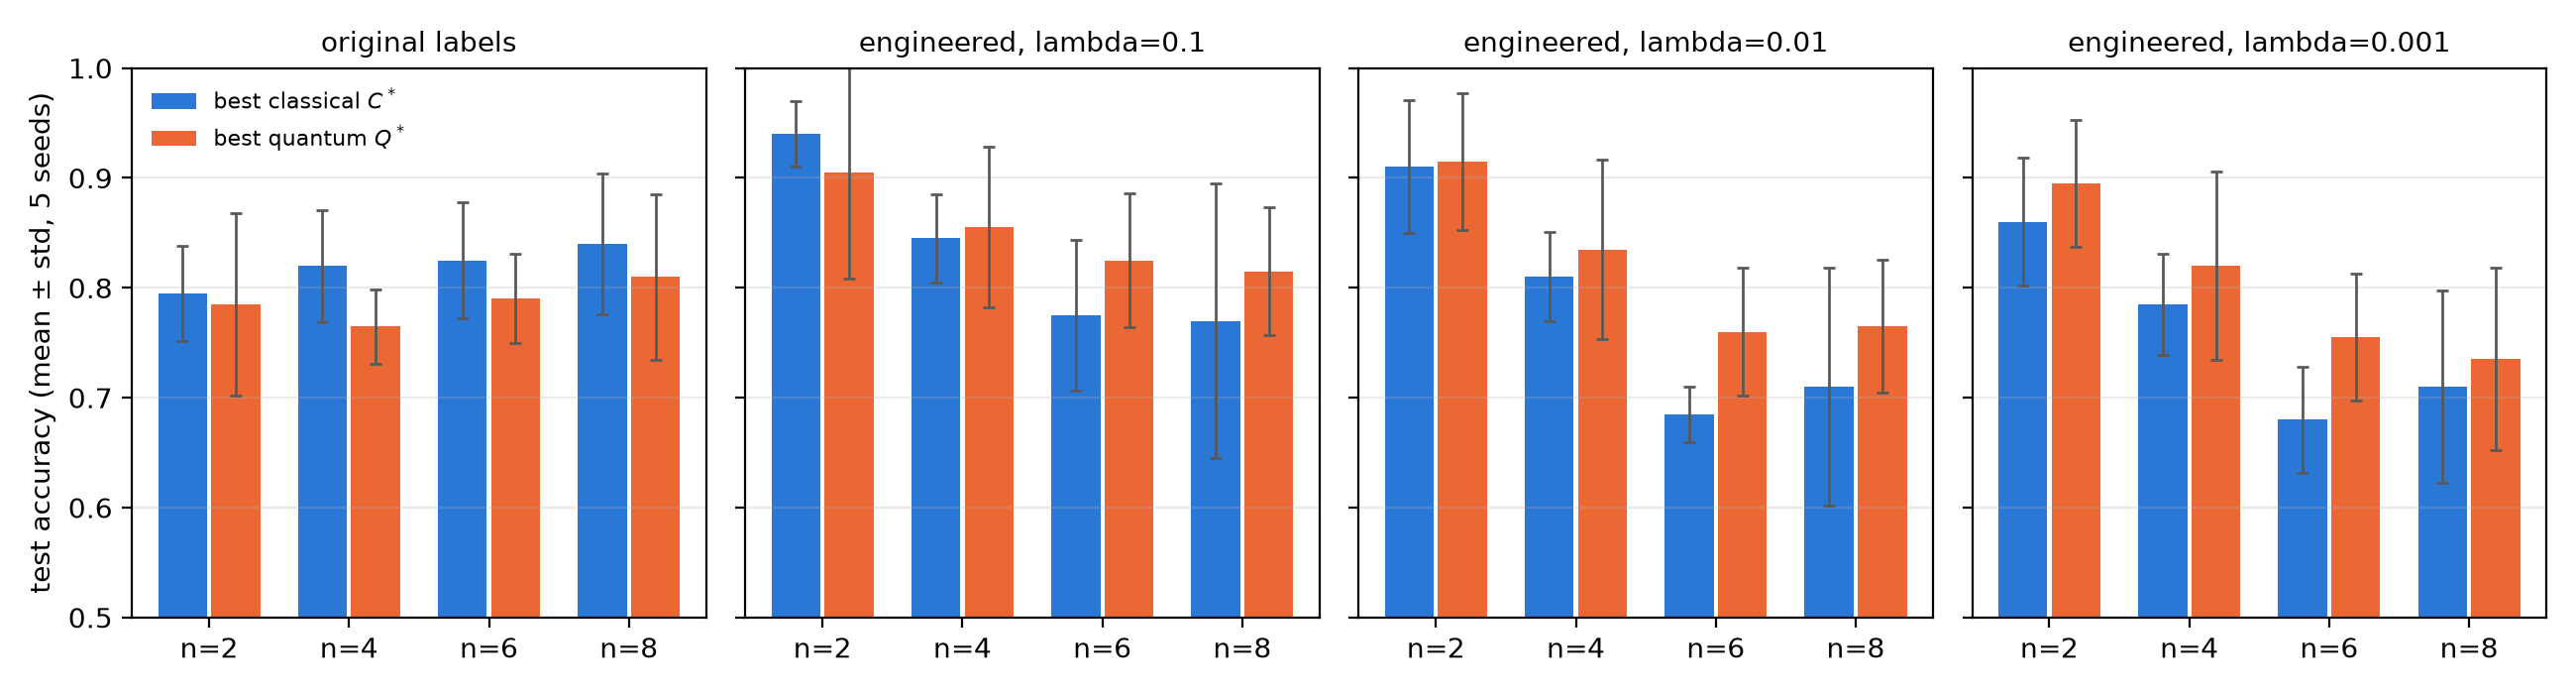
\includegraphics[width=\textwidth]{final_best_classical_vs_best_quantum.png}
\caption{Best classical model $C^\ast$ vs.\ best quantum model $Q^\ast$ (both chosen by training CV), test accuracy, mean $\pm$ std over 5 seeds. Left: original labels. Right three panels: engineered labels for the three generator values of $\lambda$.}
\label{fig:bars}
\end{figure*}

Table~\ref{tab:orig} and Fig.~\ref{fig:bars} (left) show the original-label results. Every model clears the majority-class floor, and the label-shuffle check (tuned RBF SVM on permuted labels) gives a mean test accuracy of 0.501 over the 20 seed--qubit runs, so this check found no evidence of label leakage. $C^\ast$ is the RBF SVM in 14 of 20 runs, the polynomial SVM in 5 and the linear SVM in 1. The sampled $L=2$ fidelity kernel is below its classically computable $L=1$ version at $n=4,6,8$ and above it by one test image (over five seeds) at $n=2$; its gap to $C^\ast$ is positive only at $n=2$ ($+0.035\pm0.049$), without meeting the criterion. The projected kernel is 0.010--0.100 below $C^\ast$. $Q^\ast$ is the projected kernel in 4, 2, 0 and 1 of the 5 seeds at $n=2,4,6,8$, and is below $C^\ast$ at every $n$ ($\Delta A^\ast$ from $-0.055$ to $-0.010$). In a shot study at $n=4$ the fidelity-kernel error falls as $1/\sqrt{\text{shots}}$ (0.0173 at 256 shots to 0.0030 at 8192) while test accuracy stays at 0.790--0.795 from 1024 shots on, so 2048 shots suffice.

\subsection{Geometric difference}

\begin{table}[t]
\centering
\caption{$g_{\mathrm{gen}}$ at $\lambda=0.1$ (training images, ideal quantum kernels), mean over 5 seeds.}
\label{tab:g}
\footnotesize
\begin{tabular}{@{}lcccc@{}}
\toprule
Pair & $n=2$ & $n=4$ & $n=6$ & $n=8$ \\
\midrule
Projected vs.\ RBF & 2.68 & 2.95 & 3.23 & 3.01 \\
Projected vs.\ polynomial & 2.88 & 2.97 & 3.49 & 4.15 \\
Projected vs.\ linear$^{a}$ & 0.64 & 0.96 & 0.90 & 1.21 \\
Projected vs.\ $C^\ast$ & 3.02 & 2.95 & 3.56 & 3.19 \\
\midrule
Fidelity vs.\ RBF & 2.61 & 2.83 & 2.45 & 2.35 \\
Fidelity vs.\ polynomial & 2.90 & 2.80 & 3.89 & 3.90 \\
Fidelity vs.\ linear$^{a}$ & 0.57 & 0.94 & 1.24 & 1.28 \\
Fidelity vs.\ $C^\ast$ & 2.87 & 2.83 & 3.54 & 2.81 \\
\bottomrule
\end{tabular}
\\[2pt]{\footnotesize $^{a}$Not comparable: the linear kernel has rank at most $n$, and its $g_{\mathrm{tra}}$ is 2.96--7.47, so the regularisation dominates.}
\end{table}

Against the RBF, polynomial and $C^\ast$ kernels, $g_{\mathrm{gen}}$ lies between 2.35 and 4.15 for both quantum kernels, with no clear trend in $n$ (Table~\ref{tab:g}). The small values against the linear kernel are an artifact of regularisation ($g_{\mathrm{tra}}$ of 2.96--7.47, against 0.35--1.99 for the other pairs). $g_{\mathrm{gen}}$ depends on $\lambda$: against $C^\ast$ its mean is 9.4--24.3 (projected) and 4.5--16.7 (fidelity) at $\lambda=10^{-3}$, and 1.2--1.9 at $\lambda=1$; Huang's rule can be met in only 15 of 60 projected and 27 of 60 fidelity pairs.

\begin{figure*}[t]
\centering
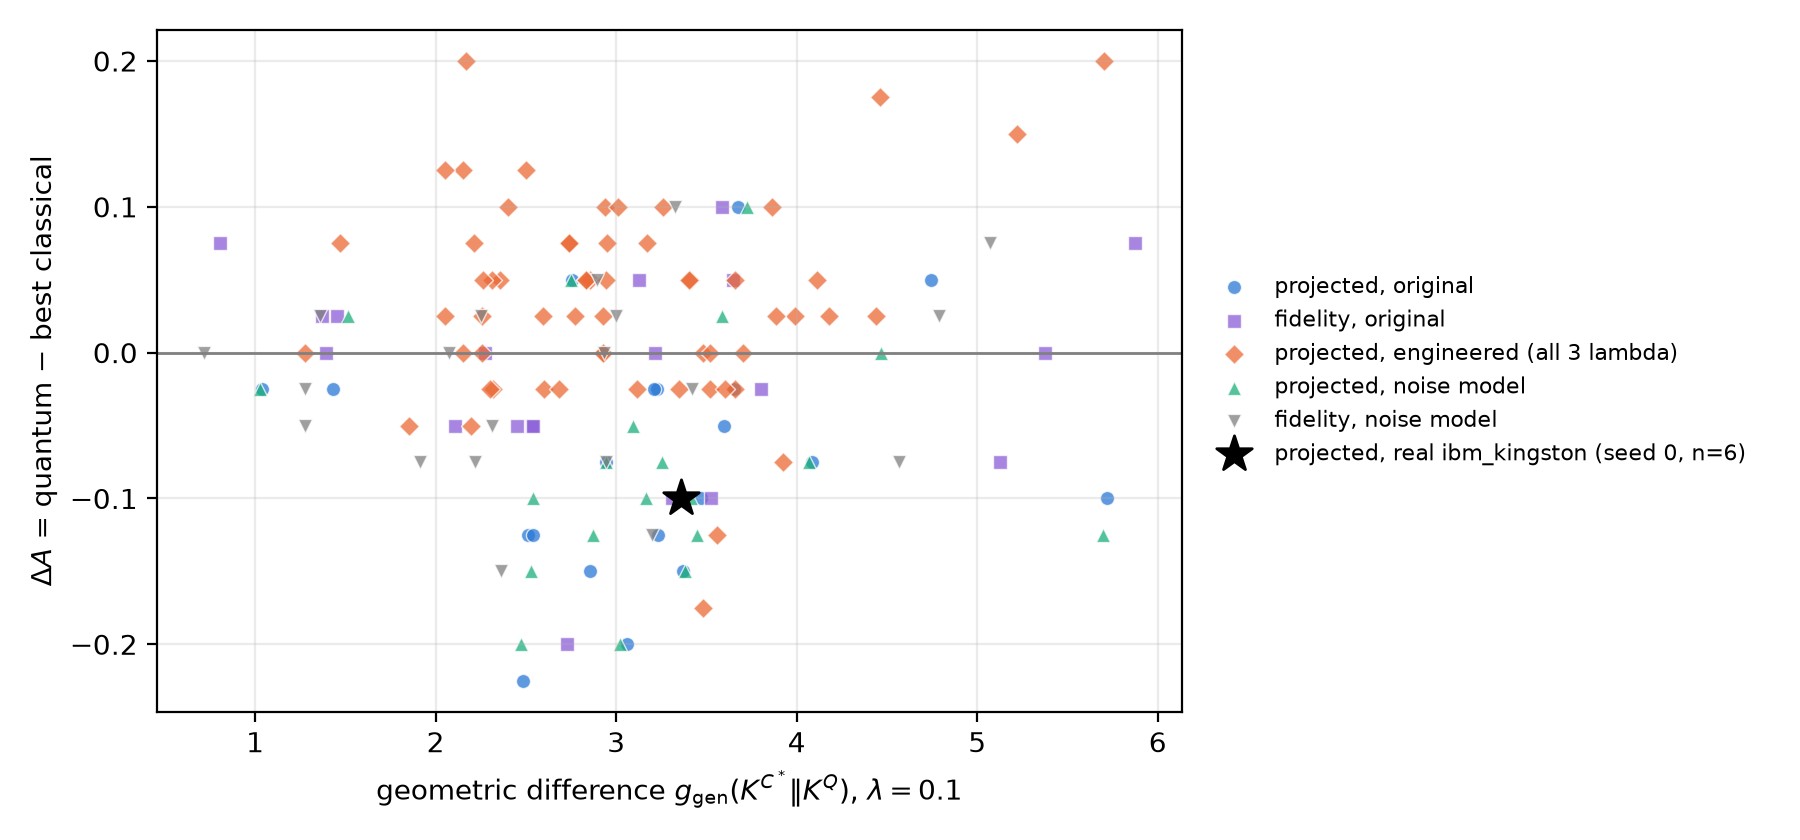
\includegraphics[width=0.62\textwidth]{final_deltaA_vs_g_all.png}
\caption{Accuracy gap $\Delta A$ vs.\ $g_{\mathrm{gen}}(K^{C^\ast}\|K^Q)$ at $\lambda=0.1$ for every setting we ran: one point per seed and qubit count (and per $\lambda$ for engineered labels). Star: the real-hardware run on the original labels (Job~1, seed 0, $n=6$).}
\label{fig:dAg}
\end{figure*}

Fig.~\ref{fig:dAg} plots $\Delta A$ against $g_{\mathrm{gen}}(K^{C^\ast}\|K^Q)$ for every setting. Within every group $g$ is a poor predictor of $\Delta A$: the correlation coefficient is $r=+0.12$ (projected, original labels, 20 runs), $-0.01$ (fidelity, original), $+0.11$ (projected, engineered, 60 runs), $-0.04$ (projected, noise model) and $+0.21$ (fidelity, noise model). What separates the groups is the labels, not $g$: for the projected kernel the mean $g$ is 3.18 on the original and 3.02 on the engineered labels, but $\Delta A>0$ in 3 of 20 runs on the original labels and in 38 of 60 on the engineered ones.

\subsection{Engineered labels}

\begin{table}[t]
\centering
\caption{Engineered labels: $\Delta A$ (sampled quantum kernel minus $C^\ast$), mean $\pm$ std over 5 seeds. $^\dagger$Meets the improvement criterion $\overline{\Delta A}>\sigma_{\Delta A}$.}
\label{tab:eng}
\scriptsize
\setlength{\tabcolsep}{2.5pt}
\begin{tabular}{@{}lcccc@{}}
\toprule
$\lambda$ & $n=2$ & $n=4$ & $n=6$ & $n=8$ \\
\midrule
\multicolumn{5}{@{}l}{\textit{Projected kernel}} \\
0.1 & $-0.035\pm0.072$ & $+0.010\pm0.041$ & $+0.050\pm0.035^\dagger$ & $+0.055\pm0.086$ \\
0.01 & $+0.020\pm0.040$ & $+0.025\pm0.052$ & $+0.075\pm0.057^\dagger$ & $+0.055\pm0.080$ \\
0.001 & $+0.035\pm0.051$ & $+0.035\pm0.049$ & $+0.075\pm0.050^\dagger$ & $+0.025\pm0.099$ \\
\midrule
\multicolumn{5}{@{}l}{\textit{Fidelity kernel}} \\
0.1 & $-0.035\pm0.075$ & $-0.015\pm0.025$ & $-0.065\pm0.060$ & $\phantom{+}0.000\pm0.079$ \\
0.01 & $-0.085\pm0.109$ & $+0.015\pm0.060$ & $+0.005\pm0.060$ & $-0.045\pm0.037$ \\
0.001 & $-0.010\pm0.041$ & $-0.005\pm0.037$ & $-0.030\pm0.029$ & $-0.040\pm0.034$ \\
\bottomrule
\end{tabular}
\end{table}

The engineered labels agree with the T-shirt/Shirt labels on 0.42--0.58 of the images (mean per $n$), so they define a new task on the same images, and a harder one for the classical models: $C^\ast$ test accuracy falls from 0.940, 0.845, 0.775, 0.770 ($\lambda=0.1$) to 0.860, 0.785, 0.680, 0.710 ($\lambda=0.001$) for $n=2,4,6,8$. The projected kernel has a positive mean gap in 11 of 12 settings and meets the improvement criterion at $n=6$ for all three $\lambda$ ($+0.050$ to $+0.075$; Table~\ref{tab:eng}, Fig.~\ref{fig:bars}); at the other qubit counts the seed-to-seed spread is as large as the gap. The fidelity kernel, which the labels were not built for, shows no improvement. $Q^\ast$ is the projected kernel in 58 of 60 engineered runs, so the best-vs-best comparison gives the same verdicts.

\subsection{Noise}

\begin{table}[t]
\centering
\caption{Original labels: test accuracy at three levels (mean over 5 seeds), $\Delta A=A^Q_{\mathrm{noisy}}-A^{C^\ast}$ (mean $\pm$ std), and $g_{\mathrm{gen}}$ vs.\ $C^\ast$ from ideal / noisy kernels.}
\label{tab:noise}
\scriptsize
\setlength{\tabcolsep}{2.2pt}
\resizebox{\columnwidth}{!}{%
\begin{tabular}{@{}lcccc@{}}
\toprule
 & $n=2$ & $n=4$ & $n=6$ & $n=8$ \\
\midrule
\multicolumn{5}{@{}l}{\textit{Projected kernel}} \\
Exact & 0.820 & 0.740 & 0.790 & 0.740 \\
Sampled & 0.785 & 0.720 & 0.750 & 0.740 \\
Noise model & 0.790 & 0.720 & 0.750 & 0.725 \\
$\Delta A$ noise model & $-0.005\pm0.103$ & $-0.100\pm0.035$ & $-0.075\pm0.057$ & $-0.115\pm0.056$ \\
$g_{\mathrm{gen}}$ ideal / noisy & 3.02/2.98 & 2.95/2.92 & 3.56/3.54 & 3.19/3.15 \\
\midrule
\multicolumn{5}{@{}l}{\textit{Fidelity kernel}} \\
Exact & 0.830 & 0.795 & 0.795 & 0.845 \\
Sampled & 0.830 & 0.790 & 0.790 & 0.810 \\
Noise model & 0.825 & 0.800 & 0.780 & 0.795 \\
$\Delta A$ noise model & $+0.030\pm0.048$ & $-0.020\pm0.033$ & $-0.045\pm0.053$ & $-0.045\pm0.076$ \\
$g_{\mathrm{gen}}$ ideal / noisy & 2.87/2.58 & 2.83/2.56 & 3.54/3.18 & 2.81/2.46 \\
\bottomrule
\end{tabular}}
\end{table}

Moving from sampled to noisy kernels changes mean test accuracy by $-0.015$ to $+0.010$ for both kernels (Table~\ref{tab:noise}); neither meets the improvement criterion under noise. The noise is visible in the kernel inputs: the projected kernel's Pauli-feature error rises from 0.014--0.016 (sampled) to 0.030--0.079 (noisy) and its mean Bloch-vector length shrinks (e.g.\ 0.919 to 0.753 at $n=2$); the fidelity-kernel error rises from 0.006 to 0.093--0.132, and the smallest eigenvalue of the noisy fidelity matrix is $-0.048$ at $n=2$ (positive at $n\ge4$; no repair). \textbf{Enhancement: noisy geometric difference.} Huang \textit{et al.} compute $g$ from ideal kernels; we also compute it from noisy ones. Noise lowers $g_{\mathrm{gen}}$ by 9--13\% for the fidelity kernel but by only 0.5--1.4\% for the projected kernel, whose geometry relative to the classical kernels is thus far more robust to device noise.

\subsection{Real hardware: four-level comparison}

\begin{table}[t]
\centering
\caption{Four-level comparison, original labels, seed 0, $n=6$, 120 images (Job~1; $C^\ast$ = polynomial SVM, 0.925). Error: mean $|\text{feature}-\text{exact}|$ over the three Paulis. Shrink: mean slope of measured vs.\ exact $\langle Z_k\rangle$ (1 = none).}
\label{tab:four}
\footnotesize
\setlength{\tabcolsep}{3.2pt}
\begin{tabular}{@{}lcccccc@{}}
\toprule
Level & Acc. & $\Delta A$ & $g_{\mathrm{gen}}$ & Error & Bloch & Shrink \\
\midrule
Exact & 0.800 & $-0.125$ & 3.37 & 0 & 0.521 & 1 \\
Sampled & 0.775 & $-0.150$ & 3.38 & 0.016 & 0.522 & 0.997 \\
Noise model & 0.775 & $-0.150$ & 3.38 & 0.030 & 0.480 & 0.912 \\
Noise model, dry run & 0.800 & $-0.125$ & 3.38 & 0.029 & 0.479 & -- \\
\texttt{ibm\_kingston} & 0.825 & $-0.100$ & 3.36 & 0.023 & 0.503 & 0.951 \\
\bottomrule
\end{tabular}
\end{table}

\begin{figure*}[t]
\centering
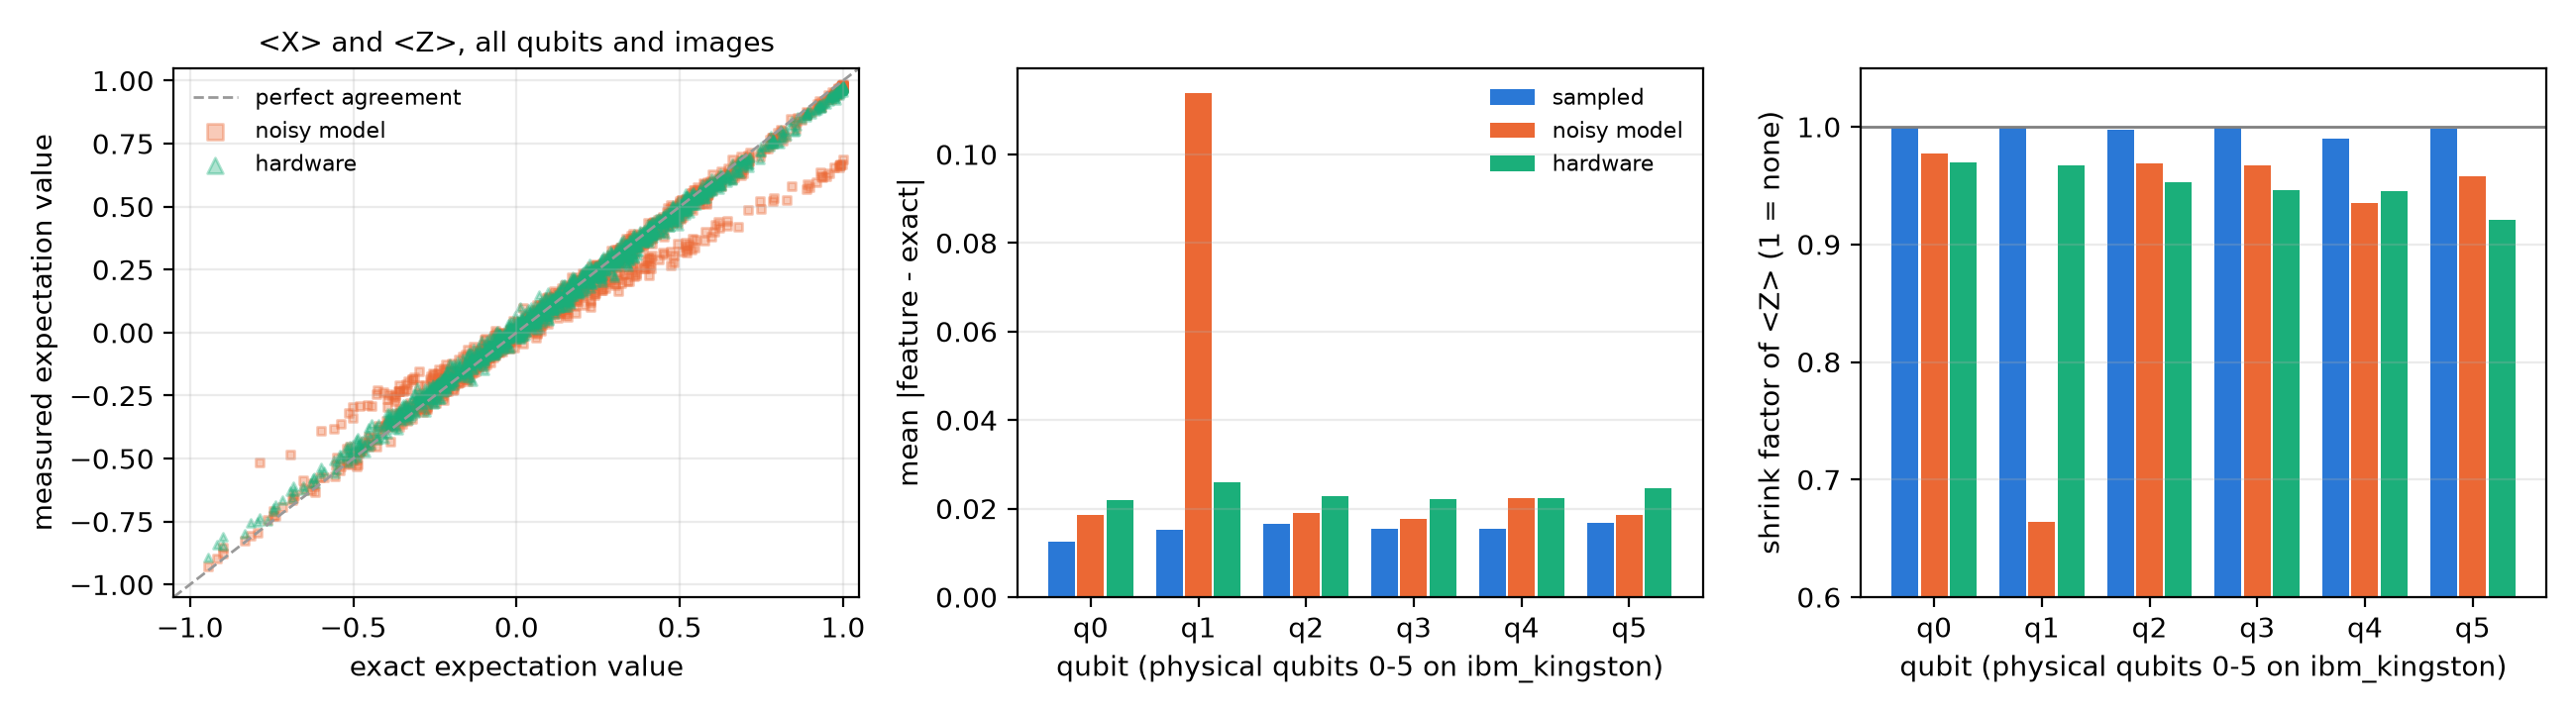
\includegraphics[width=0.84\textwidth]{four_level_features.png}
\caption{Four-level comparison of the projected-kernel features (Job~1, seed 0, $n=6$, 120 images). Left: measured vs.\ exact $\langle X_k\rangle$ and $\langle Z_k\rangle$. Middle: mean absolute error per physical qubit. Right: shrink factor of $\langle Z_k\rangle$ per qubit.}
\label{fig:four}
\end{figure*}

The real device is closer to the exact features than the noise model (Table~\ref{tab:four}, Fig.~\ref{fig:four}): feature error 0.023 against 0.030, Bloch length 0.503 against 0.480, shrink factor 0.951 against 0.912. The difference comes mainly from physical qubit 1, with a readout error of 17--18\% in the calibration snapshot but at most 2\% on the device during our run ($p_{10}\le1.1\%$, $p_{01}=1.1$--$2.0\%$ on all six qubits). On the device the errors are spread evenly (per-qubit error 0.022--0.026, shrink 0.921--0.970). The mean $\langle Y_k\rangle$, exactly 0 for our real-amplitude circuit, is $+0.0046$ on hardware (up to $+0.012$ per qubit) against $\le0.001$ in simulation, a small sign of coherent errors that the noise model does not contain. Classification is unaffected: accuracy is 0.775--0.825 at every level (the noise model and its dry run differ by one test image because they use different simulator seeds), $g$ stays at 3.36--3.38, and the gap to $C^\ast$ is $-0.100$ to $-0.150$, as in simulation.

\subsection{Did we see something? The advantage on a device}\label{sec:adv}

\begin{table*}[t]
\centering
\caption{Engineered labels, $n=6$: $\Delta A$ of the projected kernel at each level ($\alpha=1$, each level re-tuned on its own features). Left: mean $\pm$ std over 5 seeds; $^\dagger$meets the improvement criterion. Right: seed 0, the seed measured on \texttt{ibm\_kingston} (Job~2).}
\label{tab:adv}
\footnotesize
\setlength{\tabcolsep}{4.5pt}
\begin{tabular}{@{}lccc@{\hspace{14pt}}ccccc@{}}
\toprule
 & \multicolumn{3}{c}{5 seeds} & \multicolumn{5}{c}{Seed 0} \\
\cmidrule(r{10pt}){2-4}\cmidrule{5-9}
$\lambda$ & Ideal & Noise model & Noise + mitig. & Ideal & Noise model & Noise + mitig. & Hardware & Hardware + mitig. \\
\midrule
0.1 & $+0.050\pm0.035^\dagger$ & $+0.045\pm0.040^\dagger$ & $+0.040\pm0.030^\dagger$ & $+0.000$ & $+0.000$ & $+0.000$ & $-0.050$ & $-0.050$ \\
0.01 & $+0.075\pm0.057^\dagger$ & $+0.095\pm0.062^\dagger$ & $+0.080\pm0.089$ & $+0.125$ & $+0.125$ & $+0.150$ & $+0.075$ & $+0.075$ \\
0.001 & $+0.075\pm0.050^\dagger$ & $+0.060\pm0.046^\dagger$ & $+0.070\pm0.037^\dagger$ & $+0.100$ & $+0.100$ & $+0.100$ & $+0.025$ & $+0.025$ \\
\bottomrule
\end{tabular}
\end{table*}

\begin{figure*}[t]
\centering
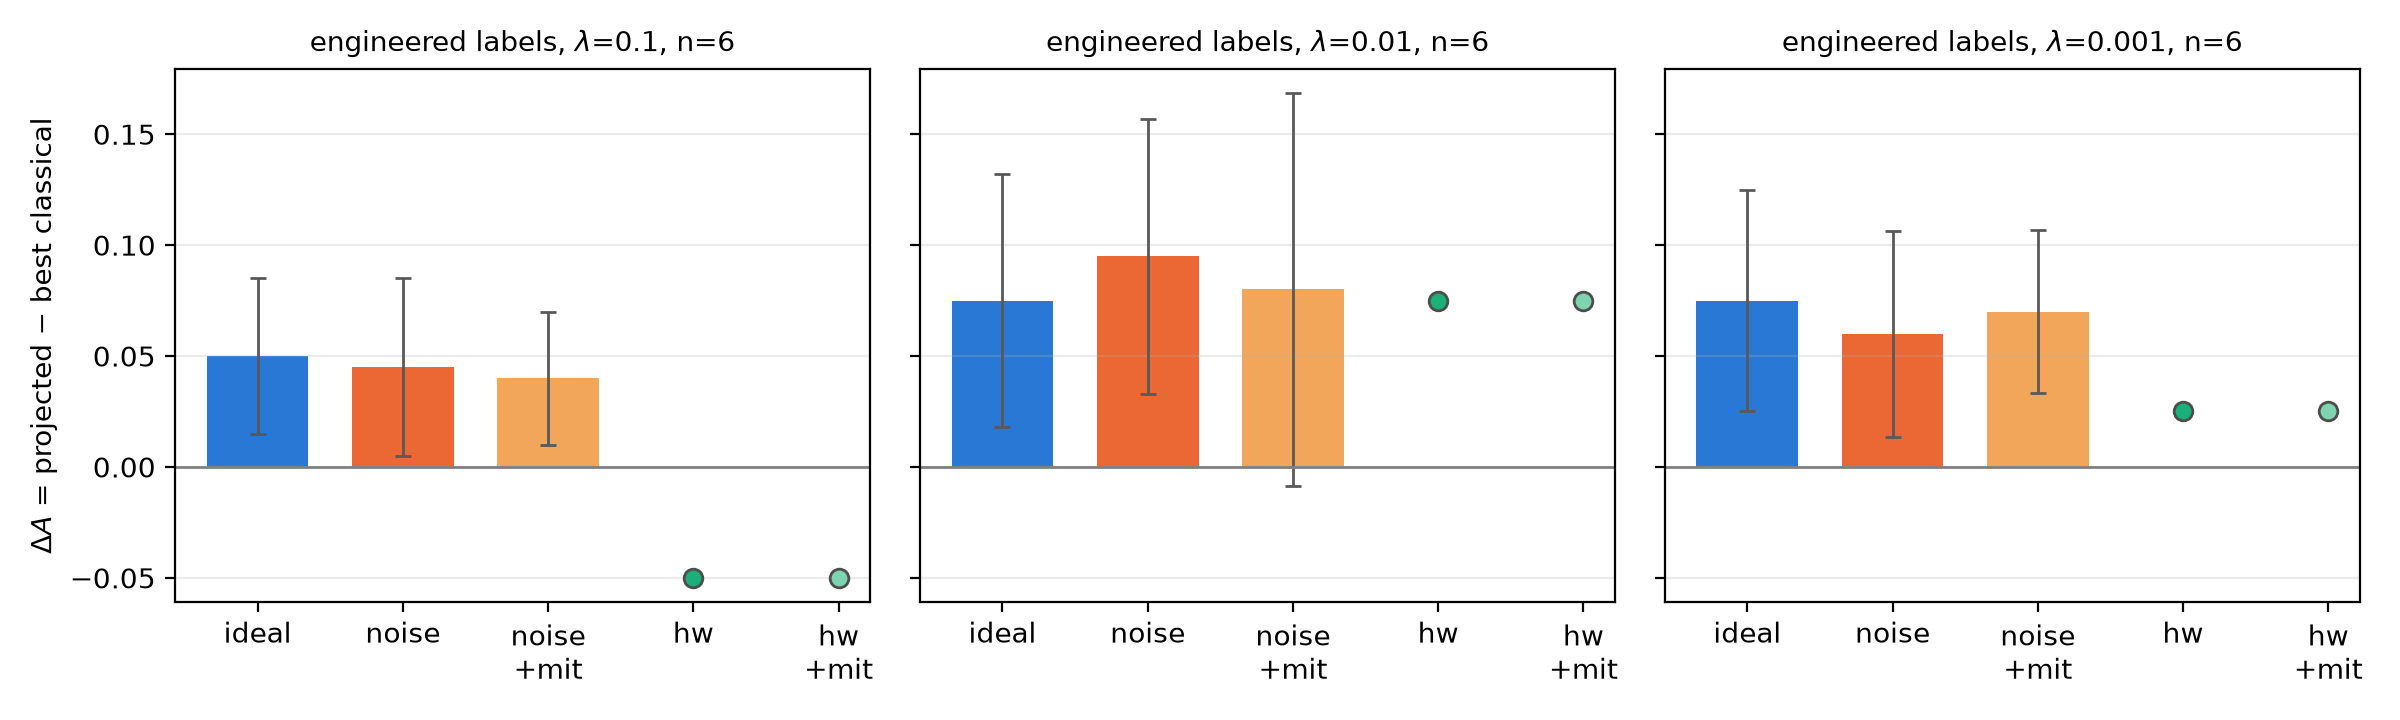
\includegraphics[width=0.84\textwidth]{advantage_under_noise.png}
\caption{Engineered labels, $n=6$: $\Delta A$ of the projected kernel at each level. Bars: mean $\pm$ std over 5 seeds (ideal, noise model, noise model with readout mitigation). Dots: seed 0 on \texttt{ibm\_kingston}, without and with readout mitigation.}
\label{fig:adv}
\end{figure*}

\textbf{Noise model (5 seeds): the advantage survives.} With the full \texttt{ibm\_kingston} noise model the projected kernel still meets the improvement criterion for all three $\lambda$ ($\overline{\Delta A}=+0.045$, $+0.095$, $+0.060$; $C^\ast$ accuracy 0.775, 0.685, 0.680; Table~\ref{tab:adv}, Fig.~\ref{fig:adv}). Readout mitigation lengthens the noisy Bloch vectors (mean 0.584 to 0.633) but does not improve accuracy: the criterion still holds for $\lambda=0.1$ and $0.001$, and the gap at $\lambda=0.01$ ($+0.080$) is now smaller than its spread ($0.089$).

\textbf{Real hardware (seed 0): the advantage shrinks.} For seed 0 the noise model reproduces the ideal result exactly ($+0.000$, $+0.125$, $+0.100$). On \texttt{ibm\_kingston} the gap drops by 0.050--0.075 to $-0.050$, $+0.075$ and $+0.025$: the projected kernel still beats $C^\ast$ for two of the three label sets, by 3 and 1 test images. Readout mitigation changes nothing, as expected with readout errors of at most 2\%. The hardware features themselves are accurate (mean error 0.023, Bloch length 0.668 against 0.690 exact, $\langle Y\rangle=+0.009$), and $g_{\mathrm{gen}}$ against $C^\ast$ is unchanged (2.11, 2.15, 3.84 on hardware against 2.15, 2.15, 3.87 ideal). The loss was visible before the test set was used: the best inner-CV accuracy on the hardware features is lower than on the ideal ones for every $\lambda$ (0.913 vs.\ 0.938, 0.913 vs.\ 0.925, 0.875 vs.\ 0.888); on the noise model it fell only for $\lambda=0.01$, where the test gap did not change.

\textbf{What this means.} The advantage is robust to the errors the noise model contains (gate errors, decoherence, large readout errors), but real hardware adds errors it does not contain; small coherent errors (non-zero $\langle Y\rangle$) and calibration drift are possible causes, not identified. With one hardware seed and 40 test images this is a single observation, not an estimated effect.

\subsection{Discussion}\label{sec:disc}
\textbf{Original labels (sub-question 1).} No quantum kernel, nor $Q^\ast$, improves on $C^\ast$ at any $n$, so falsifier (ii) is not triggered.

\textbf{Geometric difference (sub-question 2).} $g_{\mathrm{gen}}\approx3$ for both kernels against $C^\ast$: the quantum kernels are geometrically different from the classical ones, yet there is no advantage on the original labels, and $g$ is not associated with $\Delta A$ in any group of runs ($|r|\le0.21$), nor does it trend with $n$. This is consistent with Huang \textit{et al.}: a large $g$ makes an advantage \emph{possible} for some labels; it does not guarantee one for a given task.

\textbf{Engineered labels (sub-question 3).} Relabeling cannot change $g$, which depends only on the images and kernels (up to the tuned $C^\ast$). Read literally, falsifier (i) is therefore \emph{untested}, since no setting with a clearly larger $g$ exists. Read as intended in Huang \textit{et al.}'s construction, i.e.\ labels aligned with the large-$g$ direction, (i) is tested and not triggered: the projected kernel meets the improvement criterion at $n=6$ for all three $\lambda$, while the fidelity kernel, whose geometry was not used, shows none. We report both readings. The gaps are small (0.050--0.075) and the generator was chosen after one preliminary check (Week~2 report), so we treat this as weak evidence, not a demonstrated advantage.

\textbf{Shots, noise and hardware (sub-question 4).} In our shot study 2048 shots suffice; device noise changes accuracy by at most 0.015 and lowers the fidelity kernel's $g$ by about 10\% but the projected kernel's barely; on the real device the projected features are closer to exact than the noise model predicts.

\textbf{Does the advantage survive a device (sub-question 5)?} On the noise model, yes, over 5 seeds. On the real device, partly: on one seed the gap shrinks by 2--3 test images and stays positive for two of three label sets. Our answer to ``do we see something?'' is therefore: on natural labels, no; on labels built along the direction where the projected kernel differs most from every classical kernel, a small advantage appears at 6 qubits, survives the \texttt{FakeKingston} noise model, and shrinks but does not vanish on one real-hardware seed.

\textbf{Limitations.} 80/40 images per seed, 5 seeds (one on hardware for the advantage test) and a heuristic, not statistical, improvement criterion; one encoding circuit; noise from one calibration snapshot, with the noisy fidelity diagonal set to 1; engineered labels defined transductively; PCA and scaling (unsupervised, no labels) are fitted once on each outer training set and shared by the inner folds, for all models alike, so inner-CV scores are not fully independent of the validation folds. All conclusions hold only for these models, budgets and data, not for quantum kernels in general.

\section{Recommendations for QML Engineers (first draft)}\label{sec:rec}
Each follows from our results and is limited to settings like ours (kernel SVMs, 2--8 qubits, small data).
\begin{enumerate}
\item \textbf{Treat $g$ as a ceiling, not a forecast.} $g\approx3$ on both tasks, yet $\Delta A$ was negative on the natural labels and positive on the engineered ones, and $|r(g,\Delta A)|\le0.21$ in every group. Compute $g$ before spending hardware time, but do not use it to predict accuracy: the labels decide whether a task uses the difference.
\item \textbf{Fix the regulariser in advance and report its effect.} With few features $K^C$ is nearly low rank: Huang's $\lambda$ rule was feasible in only 15--27 of 60 pairs, and the mean $g$ against $C^\ast$ ranged from about 1.2 to 24 over $\lambda\in[10^{-3},1]$. Declare $\lambda$ before looking at accuracy, report $g_{\mathrm{tra}}$, and exclude low-rank kernels such as the linear kernel from $g$ comparisons.
\item \textbf{Compare at a matched budget, against the best classical model and a classical twin.} Tune every model with the same number of settings, choose $C^\ast$ and $Q^\ast$ by cross-validation, and include a classically computable version of the quantum model ($L=1$ here). Keep simple baselines too: logistic regression, not even a candidate for $C^\ast$, scored 0.840--0.850 on the natural labels, at or above $C^\ast$ at every $n$.
\item \textbf{Prefer projected kernels when hardware is the target.} They need 3 circuits per image instead of one per pair (360 vs.\ 6{,}360 circuits and 0.74 vs.\ 13.0 million shots per seed here; linear instead of quadratic growth), their matrices are PSD by construction, and their $g$ moved by at most 1.4\% under noise against 9--13\% for the fidelity kernel.
\item \textbf{Validate on real hardware, not only on a noise model.} The calibration snapshot was pessimistic about readout (17\% vs.\ at most 2\% on qubit 1) but optimistic about accuracy on the advantage task (no loss vs.\ 2--3 test images lost on seed 0). Re-tune on device features and watch their inner-CV accuracy: on hardware it fell for every label set before the test set was used (on the noise model, for one).
\item \textbf{Use low-cost diagnostics.} For a real-amplitude encoding $\langle Y\rangle$ should be 0; on hardware it was an order of magnitude larger than in simulation, a cheap indicator of coherent errors. Two readout-calibration circuits per job (2 of 362 circuits) and enable readout mitigation, which helps when readout errors are large (noise model) and does nothing for gate errors.
\item \textbf{Plan the quantum budget and protect every run.} One job of 362 circuits $\times$ 2048 shots used 197~s of a 600~s allowance per 28 days. Run the identical transpiled circuits on a noise model first, save job IDs and raw counts before any analysis, and guard submissions against the remaining quota.
\item \textbf{Report spread honestly.} With 40 test images one image is 0.025 accuracy; use several seeds, report the standard deviation, and flag single hardware runs.
\end{enumerate}

\section{Conclusion}
Under a matched tuning budget, neither quantum kernel beats the best classical model on the natural T-shirt/Shirt task at 2--8 qubits, although both are geometrically different from the classical kernels ($g\approx3$); $g$ marks a possibility, not a prediction. When the labels are built along the direction of largest geometric difference, the projected kernel shows a small advantage at 6 qubits that survives the \texttt{FakeKingston} noise model and shrinks, but does not vanish, on one seed on the real \texttt{ibm\_kingston} device. For this circuit and data size the projected kernel is the practical choice for hardware: far cheaper, PSD by construction, and with a $g$ that our noise model barely changes. \textbf{Remaining work (Week~4, Dec.~6):} a second hardware seed for the advantage test if quota allows (204~s remain; the last job used 197~s, so one more job fits only just), final recommendations, the final report and presentation, and a tagged GitHub release.

\section{Changes since Week 2}\label{sec:changes}
\begin{itemize}
\item \textbf{Professor's feedback:} circuit diagrams of both kernel architectures and the hardware circuit (Section~\ref{sec:circ}); the advantage tested on a noise model and real hardware (Sections~\ref{sec:advexp}, \ref{sec:adv}); recommendations for QML engineers (Section~\ref{sec:rec}).
\item \textbf{Hardware plan expanded:} all 120 images of a seed at 2048 shots (the shot count of every other level), instead of about 10 images at about 4{,}000 shots, so the hardware features feed the classifier; two jobs instead of one. Job~2 uses $\alpha=1$ because the advantage test needs it (Section~\ref{sec:hw}).
\item \textbf{New analyses:} best classical vs.\ best quantum ($Q^\ast$), $\Delta A$ vs.\ $g$ across all settings, readout mitigation, re-tuning on device features (Section~\ref{sec:advexp}), and resource counts with shots (Table~\ref{tab:res}).
\item \textbf{Reproducibility:} re-running notebooks 01, 03--05 and 07--11 on Linux reproduced every reported number except one: at seed 0, $n=4$, two projected-kernel settings tied in inner CV and a one-count platform difference in shot sampling changed the pick, which would move the $n=4$ projected mean from 0.720 to 0.735. Reported numbers come from the saved files, and the README shows how to reproduce each.
\end{itemize}

\section*{Author Contributions}
F.~Shahzad: shared data and evaluation code, encoding circuit, fidelity kernel with qubit and shot studies, IBM hardware code and both hardware jobs. S.~ul~Arifeen: projected-kernel features and kernel, noise model and noisy geometric difference, four-level comparison, best-vs-best analysis, advantage-under-noise test. H.~Nadeem: classical baselines and matched budget, geometric difference, engineered dataset, circuit diagrams. All authors contribute to the report and presentation.

\begin{thebibliography}{4}
\bibitem{huang2021} H.-Y. Huang, M. Broughton, M. Mohseni, R. Babbush, S. Boixo, H. Neven, and J. R. McClean, ``Power of data in quantum machine learning,'' \textit{Nat. Commun.}, vol. 12, p. 2631, 2021.
\bibitem{schuld2019} M. Schuld and N. Killoran, ``Quantum machine learning in feature Hilbert spaces,'' \textit{Phys. Rev. Lett.}, vol. 122, p. 040504, 2019.
\bibitem{havlicek2019} V. Havl\'{i}\v{c}ek \textit{et al.}, ``Supervised learning with quantum-enhanced feature spaces,'' \textit{Nature}, vol. 567, pp. 209--212, 2019.
\bibitem{xiao2017} H. Xiao, K. Rasul, and R. Vollgraf, ``Fashion-MNIST: a novel image dataset for benchmarking machine learning algorithms,'' arXiv:1708.07747, 2017.
\end{thebibliography}

\end{document}
